%%
% Please see https://bitbucket.org/rivanvx/beamer/wiki/Home for obtaining beamer.
%%
\documentclass[notes]{beamer}
%\documentclass[notes=hide]{beamer}
%\documentclass[notes=only]{beamer}

\usetheme{Madrid}

\setbeamertemplate{footline}
{
	\leavevmode%
	\hbox{%
		\begin{beamercolorbox}[wd=.333333\paperwidth,ht=2.25ex,dp=1ex,center]{author in head/foot}%
			\usebeamerfont{author in head/foot}\insertshortauthor%~~\beamer@ifempty{\insertshortinstitute}{}{(\insertshortinstitute)}
		\end{beamercolorbox}%
		\begin{beamercolorbox}[wd=.333333\paperwidth,ht=2.25ex,dp=1ex,center]{title in head/foot}%
			\usebeamerfont{title in head/foot}\insertshorttitle
		\end{beamercolorbox}%
		\begin{beamercolorbox}[wd=.333333\paperwidth,ht=2.25ex,dp=1ex,right]{date in head/foot}%
			\insertframenumber{} / \inserttotalframenumber\hspace*{2ex} 
	\end{beamercolorbox}}%
	\vskip0pt%
}

\author{Matthew Barulic}

\title{STL}

\subtitle{C++'s Standard Containers Library}

\institute{
RoboJackets\\
Spring Training Series\\
Georgia Tech
}

\setbeamertemplate{navigation symbols}{}%hide navigation symbols

\usecolortheme[named=blue]{structure}

\AtBeginSection[]{
	\begin{frame}
	\vfill
	\centering
	\begin{beamercolorbox}[sep=8pt,center,shadow=true,rounded=true]{title}
		\usebeamerfont{title}\insertsectionhead\par%
	\end{beamercolorbox}
	\vfill
\end{frame}
}

\begin{document}

\begin{frame}
	\titlepage
\end{frame}

\begin{frame}{Today's Plan}

\tableofcontents

%\begin{itemize}
%	\item Introduce the STL
%	\item Understand cppreference.com
%	\item Review common containers
%	\item Review common algorithms
%	\item A few miscellaneous bits
%\end{itemize}
	
\end{frame}

\section{Introduction to the STL}

\begin{frame}{Brief History}
	\begin{itemize}
		\item 1979 - C++ Invented
		\item 1992 - STL Created
		\item 1998 - First Standardization
	\end{itemize}
\end{frame}

\begin{frame}{The STL}
	\textbf{S}tandard \textbf{T}emplate \textbf{L}ibrary
	\begin{itemize}
		\item Containers
		\item Iterators
		\item Algorithms
		\item Function Objects
	\end{itemize}
\end{frame}

\begin{frame}{The STL}
	Algorithms $\rightarrow$ Iterators $\rightarrow$ Containers
\end{frame}

\begin{frame}{Containers}
	\begin{itemize}
		\item Store data (objects / primitives)
		\item The \textit{Data Structures} of \\Data Structures and Algorithms (CS 1332)
		\item Minimal member methods for managing contents
	\end{itemize}

	\bigskip

	\begin{center}
		\url{http://en.cppreference.com/w/cpp/container}
	\end{center}
\end{frame}

\begin{frame}{Iterators}
	\begin{itemize}
		\item Interface for useful container operations
		\item Exposed through begin() / end() \\
			\textcolor{darkgray}{(and their variants)}
	\end{itemize}
	
	\bigskip
	
	\begin{center}
		\url{http://en.cppreference.com/w/cpp/iterator}
	\end{center}
\end{frame}

\begin{frame}{Iterators}
	\begin{figure}
		\centering
		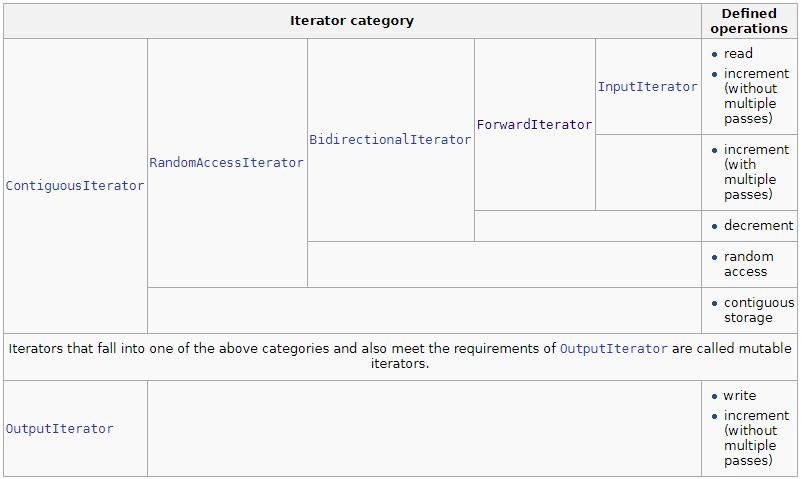
\includegraphics[width=\linewidth]{IteratorTypes}
	\end{figure}
\end{frame}

\begin{frame}{Algorithms}
	\begin{itemize}
		\item Utility functions for ranges of elements
		\item Decoupled from specific containers
	\end{itemize}
	
	\bigskip
	
	\begin{center}
		\url{http://en.cppreference.com/w/cpp/algorithm}
	\end{center}
\end{frame}

\begin{frame}{Algorithms}
	Categories of Algorithms
	\begin{itemize}
		\item Non-Modifying
		\item Modifying
		\item Sorting / Partitioning
		\item Numeric
	\end{itemize}
\end{frame}

\section{How to read cppreference.com}

\begin{frame}{cppreference.com}
	\begin{center}
		\url{http://en.cppreference.com}
	\end{center}
\end{frame}

\note[itemize]{
	\item Guided tour through std::vector's cppreference page.
	\item Constructors
	\item Member Functions
	\item Example
}

\section{Common Containers}

\begin{frame}[fragile]{array}
	\begin{itemize}
		\item Fixed size container
		\item Preferred over "c-style" arrays
		\item Two template arguments: \textit{type} and \textit{size}
	\end{itemize}
	\bigskip
	\begin{exampleblock}{Example}
	\begin{verbatim}
		std::array<int,5> my_array = {0,1,2,3,4};
	\end{verbatim}
	\end{exampleblock}
\end{frame}

\begin{frame}{vector}

\end{frame}

\begin{frame}{set}

\end{frame}

\begin{frame}{map}

\end{frame}

\section{Common Algorithms}

\begin{frame}{any\textunderscore of / all\textunderscore of / none\textunderscore of}

\end{frame}

\begin{frame}{copy}

\end{frame}

\begin{frame}{fill}

\end{frame}

\begin{frame}{generate}

\end{frame}

\begin{frame}{accumulate}

\end{frame}

\begin{frame}{transform}

\end{frame}

\section{Code Examples}

\note[itemize]{
	\item TODO a handful of simple, but not trivial examples
}

\end{document}
